\subsection{What is a probability?}
It is a \tB{mathematical measure of the uncertainty} of a given event.

\paragraph{Objectivist interpretation \cite{wiki:probability_interpretation}}: assigns
numbers describing some objective state, \tB{\textit{Frequentist} interpretation claiming
that the probability of a random event is quantified by the relative frequency in a given
experiment}. 

\paragraph{Subjectivist interpretation \cite{wiki:probability_interpretation}}: assigns
numbers quantifying the degree of belief that a given event occurs. \textit{Bayesian} 
interpretation uses expert knowledge considered as subjective and represented by the 
prior, as well as experimental data represented by the likelihood. The normalized product
of the 2 above quantity is the \tB{posterior probability distribution containing both 
expert knowledge and experimental data}.


\subsection{Properties}
\paragraph{Event and its opposite}
$\Prob{A} + \Prob{\overline{A}} = 1$
\paragraph{Not necessary mutually exclusive events}
$\Prob{A\cup B} = \Prob{A} + \Prob{B} - \Prob{A\cap B}$
\paragraph{Independent events}
$\Prob{A\cap B} = \Prob{A} \times \Prob{B}$
\paragraph{Conditional Probability}
$\probC{A}{B} = \dfrac{\prob{A\cap B}}{\prob{B}}$
\paragraph{Law of Total Probability}
$
\begin{cases}
    \left(B_{i}\right)_{1\leq i\leq n}\text{: partition of a sample }\mathcal{S}\\
    \forall i\in \inter{1}{n},~\Prob{B_{i}} \neq 0
\end{cases} 
\Rightarrow \prob{A} = \su{i=1}{n}\prob{B_{i}}\probC{A}{B_{i}}
$


\paragraph{Bayes' Theorem}
Using \tB{Law of Total Probability}:\\
$
\begin{cases}
    \left(B_{i}\right)_{1\leq i\leq n}\text{: partition of a sample }\mathcal{S}\\
    \forall i\in \inter{1}{n},~\Prob{B_{i}} \neq 0
\end{cases} 
\Rightarrow \probC{B_{i}}{A} = \dfrac{\prob{B_{i}}\times\probC{A}{B_{i}}}{\su{k=1}{n}\prob{B_{k}}\probC{A}{B_{k}}}
$


\subsection{Moments}
They are certain quantitative measures related to the shape of the function's graph.
\cite{wiki:moments_mathematics}
\paragraph{$n^{th}$ moments of a random variable:}
The $n^{th}$ moment about the origin of a random variable $X$ as denoted by
$E\left( X^{n} \right)$, is defined to be:
\begin{center}
	$\E{X^{n}}=
	\begin{cases}
		\su{x\in R_{X}}{{}}x^{n}f(x)\text{ if }X\text{ is discrete}\\
		\Su{-\infty}{\infty}x^{n}f(x)dx\text{ if }X\text{ is continuous}
	\end{cases}$
\end{center}

\paragraph{Expected value:}
The expected value of a random variable $X$ as denoted by
$E\left( X \right)$, is defined to be:
\begin{center}
	$\E{X}=
	\begin{cases}
		\su{x\in R_{X}}{{}}xf(x)\text{ if }X\text{ is discrete}\\
		\Su{-\infty}{\infty}xf(x)dx\text{ if }X\text{ is continuous}
	\end{cases}$
\end{center}
After normalized this moment by total mass we have the \tB{center of mass}.


\paragraph{Variance :}
Let $X$ be a random variable with mean $\mu_{X}$. The variance of $X$ 
denoted by $\V{X}$ or $\sigma_{X}^{2}$ is defined by:
\begin{center}
	$\V{X}=\E{\left[ X-\mu_{X} \right]^{2}}$
\end{center}
After normalized this moment by total mass we have the \tB{moment of inertia}.\\
If $X$ is a random variable with mean $\mu_{X}$ and variance $\sigma_{X}^{2}$ then:
\begin{center}
$\sigma_{X}^{2}=\E{X^{2}}-\mu_{X}^{2}$
\end{center}
And:
\begin{center}
	$\V{aX+b}=a^{2}\V{X}$
\end{center}

\paragraph{Skewness and Kurtosis}
\begin{itemize}
    \item \tB{Skewness}: $\E{\left[ \dfrac{X-\mu_{X}}{\sigma_{X}} \right]^{3}}$, indicates
        the direction (negative $\rightarrow$ left tail is longer, positive $\rightarrow$ 
        right tail is longer) and relative magnitude of a distribution's \uB{deviation from
        the normal distribution}.
    \item \tB{Kurtosis}: $\E{\left[ \dfrac{X-\mu_{X}}{\sigma_{X}} \right]^{4}}$, \uB{measures
        the outliers}, data within one standard deviation will not contribute a lot to the 
        kurtosis values conversely data exceeding one standard deviation will contribute a
        lot because of the fourth power.
\end{itemize}


\subsection{Asymptotic properties}

\paragraph{Chebychev inequality}
allows to find an estimate of the area between the
values $\mu-k\sigma\text{ and }\mu+k\sigma$ for some given $k\neq 0$, showing
that the area under $f(x)$ on the interval $\left[\mu-k\sigma, \mu+k\sigma
\right]$ is at least $1-k^{2}$.\\
Let $X$ be a random variable with probability density function $f(x)$. If
$\mu$ and $\sigma>0$ are the mean and standard deviation of $X$ then:
\begin{center}
	\fr{$\Prob{|X-\mu|<k\sigma}\geq 1-\frac{1}{k^{2}}$}
\end{center}
\begin{figure}[H]
	\begin{center}
		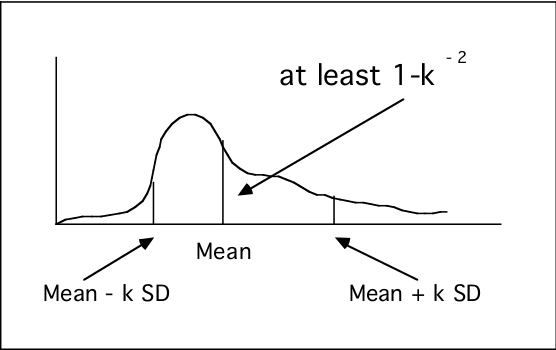
\includegraphics[width=.5\textwidth]{chapters/2_statistics/01_fundamental_probability_concepts/1_images/1_ineqChebyGraph.png}
	\end{center}
	\caption{Illustration of Chebychev inequality}
	\label{fig:fig2.01.1}
\end{figure}



\paragraph{Markov inequality}
\begin{center}
		$X\neq\underline{0}\Rightarrow \Prob{X\geq t}\leq \dfrac{\E{X}}{t}$
\end{center}
\paragraph{Theorem weak law of large numbers:}
Let $\prth{X}{i}{1}{n}\text{: independent \& identically distributed RV}$
\begin{center}
    \fr{$\forall \epsilon \in \mathbb{R}_{+}: \lm{n}{\infty}\Prob{\left|\overline{S}_{n}-\mu\right|
            \geq \epsilon}=0$ with $\overline{S}_{n}=\dfrac{1}{n}\su{ {i=1}}{n}X_{i}$}
\end{center}
\paragraph{Convergence in probability}
Suppose $\prth{X}{i}{1}{n}$ is a sequence of random variables de-
fined on a sample space S. The sequence ``converges in probability'' to the
random variable X if, for any $\epsilon>0$
\begin{center}
	$\lm{n}{\infty}\Prob{\left|X_{n}-X\right|<\epsilon}=1$
\end{center}
\paragraph{Convergence almost surely}
Suppose the RV $X\text{ and }\prth{X}{i}{1}{n}$ is a sequence of random variables de-
fined on a sample space S. The sequence $X_{n}(\omega)$ ``converges almost surely'' to $X(\omega)$ if
\begin{center}
	$\Prob{w\in S|\lm{n}{\infty}X_{n}(\omega)=X(\omega)}=1$
\end{center}
\paragraph{Properties}
\begin{itemize}
	\item For a Bernoulli distribution, $\overline{S}_{n}\text{ converges in probability to }p$
	\item For a Normal distribution, $\overline{S}_{n}\text{ converges almost surely to }\mu$
\end{itemize}


\subsection{Central Limit Theorem}
The central limit therorem (Lindeberg-Levy Theorem) states that for any
population distribution, the distribution of the standardized sample mean
is approximately standard normal with better approximations obtained with
the larger sample size.
\begin{center}
    \tR{$\begin{cases}\prth{X}{i}{1}{n}\hookrightarrow ?(\mu,\sigma^{2})\\ n\rightarrow\infty
        \end{cases} \Rightarrow \dfrac{\overline{X}-\mu}{\frac{\sigma}{\sqrt{n}}} \hookrightarrow 
    \mathcal{N}(0, 1)$}
\end{center}
\subsection{Convergence in distribution}
Consider $X$ with its cumulative density function $F$ and $\prth{X}{i}{1}{n}$ with their 
cdf $\left( F_{i} \right)_{1\leq i\leq n}$:
\begin{center}
	$\lm{n}{\infty}F_{n}(x)=F(x)\Rightarrow X_{n}\text{ "converges in distribution" to }X$
\end{center}
\subsection{Lévy Continuity Theorem}
\begin{center}
	$
	\begin{cases}	
		\prth{X}{i}{1}{n}\text{RV}\\
		\prth{F}{i}{1}{n}\text{distribution functions}\\
		\left( M_{X_{i}} \right)_{1\leq i\leq n}\text{moment generating function}
	\end{cases}$
	$\forall t\in [-h,h]\lm{n}{\infty}M_{X_{n}}(t)=M_{X}(t)\Rightarrow
	\lm{n}{\infty}F_{n}(x)=F(x)
	$
\end{center}

\section{Bivariate case}
\paragraph{Joint probability density function}
Let $\left(X,Y\right):\left(\Omega_{X},\Omega_{Y}\right)\rightarrow\left(R_{X},R_{Y}\right)$ and $f:R_{X}\times R_{Y}\rightarrow \mathbb{R}$
\begin{center}
	$\forall (x,y)\in R_{X}\times R_{Y},f(x,y)=\Prob{X=x,Y=y}\Leftrightarrow\text{ f is the joint probability density function for }X\text{ and }Y$
\end{center}

\paragraph{Marginal probability density function}
Let for all $(x,y)\in R_{X}\times R_{Y}$: $f(x,y)$ be the joint probability density of $X$ and $Y$
\begin{center}
$\begin{cases}
	f_{X}(x)=\Su{{-\infty}}{\infty}f(x,y)dy\text{is the marginal probability density of }X\\
	f_{Y}(y)=\Su{{-\infty}}{\infty}f(x,y)dx\text{is the marginal probability density of }Y
\end{cases}$
\end{center}
\paragraph{Joint cumulative probability distribution function}
Let $F:\mathbb{R}^{2}\rightarrow\mathbb{R}$
\begin{center}
	$\forall (x,y)\in \mathbb{R}^{2},F(x,y)=\Prob{X\leq x,Y\leq y}=\Su{ {-\infty}}{y}\Su{ {-\infty}}{x}f(u,v)dudv\Leftrightarrow\text{ F is the joint cumulative probability density function for }X\text{ and }Y$
\end{center}
From the fundamental theorem of calculus:
$f(x,y)=\dfrac{\partial^{2}F(x,y)}{\partial x\partial y}$


\paragraph{Conditional expectation}
The conditional mean of $X$ given $Y=y$ is defined as:
\begin{center}
\fr{
$
\E{X|y}=
\begin{cases}
\su{{x\in R_{X}}}{}xg(x/y)\Leftarrow X\text{ discrete}\\
\Su{{-\infty}}{\infty}xg(x/y)dx\Leftarrow X\text{ continuous}
\end{cases}
$}
\end{center}

Properties:
\begin{center}
	$\begin{cases}
        \mathbb{E}_{X}\left(\mathbb{E}_{y|x}\left(Y|X\right)\right)=
        \mathbb{E}_{y}\left(Y\right)\\
	\E{Y|\left\{ X=x \right\}}=\mu_{Y}+\rho\dfrac{\sigma_{Y}}{\sigma_{X}}(x-\mu_{X})
	\end{cases}$	
\end{center}


\paragraph{Conditional Variance}
\begin{center}
	$\begin{cases}
	\V{Y|x}=\E{Y^{2}|x}-\E{Y|x}^{2}\\
	\mathbb{E}_{x}\left( \V{Y|X}=(1-\rho^{2})\V{Y} \right)
	\end{cases}$
\end{center}


\paragraph{Conditional Independence}
$X\perp Y[Z \Leftrightarrow \prob{X,Y|Z}=\prob{X|Z}\prob{Y|Z}$

\paragraph{The chain rule of conditional probabilities}
Any joint probability distribution over many random variables may be decomposed into conditional
distribution over only one variable:
\begin{center}
    $\prob{x_{1:T}} = \prob{x_{1}}\prd{t=2}{T}\prob{x_{t}|x_{1:t-1}}$
\end{center}


